\documentclass[12pt]{article}

% The geometry package allows for easy page formatting.
\usepackage{geometry}
\geometry{letterpaper}

% Load up special logo commands.
\usepackage{doc}

% Package for formatting URLs.
\usepackage{url}

% Packages and definitions for graphics files.
\usepackage{graphicx}
\usepackage{epstopdf}
\usepackage{natbib}
\usepackage{tikz}
\DeclareGraphicsRule{.tif}{png}{.png}{`convert #1 `dirname #1`/`basename #1 .tif`.png}

%
% Set the title, author, and date.
%
\title{Panthera: Caching in Distributed Computing Systems}
\author{Dhaivat Pandya \\ Appleton North High School}
\date{}
%
% The document proper.
%
\begin{document}

% Add the title section.
\maketitle

% Add an abstract.
\abstract{
	The adoption of distributed computing systems has grown massively in the past few years. In particular, Apache Hadoop, which allows developers to create applications that run on a cluster of computers, is currently used throughout academia and industry. However, the Hadoop File System fails to effectively utilize memory and local storage in order to reduce waiting time (i.e. latency). Thus, there is a very significant wastage of available computational resources. In this project, a system, named Panthera, was developed which reduces waiting time and conserves computational resources by using \textit{caching}, i.e. retaining downloaded files in local memory rather than discarding them, thereby reducing access time. Panthera caches both information about files (i.e. metadata) and the file contents (i.e. data). It runs with an unmodified version of Hadoop, meaning that it can integrate easily into existing architecture. Panthera was tested using both single node and multi-node setups. The results showed a 90.8\% decrease in waiting time with the Panthera metadata cache and a 95.7\% decrease with the Panthera data cache. Such drastic decreases in latency can greatly increase the efficiency of existing Hadoop applications and also allow the creation of algorithms that were previously not feasible. Panthera has numerous applications in fields ranging from bioinformatics and medicine to market research.  All code associated with this project will be open sourced to further development in the area of distributed computing.
}

\section{Introduction}
As computational problems and their associated datasets have grown in size, it has become necessary to take advantage of distributed computing systems to solve them. Such systems allow programs to scale from one computer (i.e. one \textit{node}) to thousands of computers with few or no changes in the codebase. In particular, the Hadoop distributed system \cite{hadoop} has seen tremendous growth. Hadoop is an open source version of the revolutionary MapReduce system developed at Google \cite{mapreduce}. With it, developers can easily take advantage of large, multi-node clusters to solve computational problems.

In order to run algorithms across a network of computers, access to the dataset must be available to all nodes within a network. To facilitate this, Hadoop uses the Hadoop Distributed File System (HDFS) \cite{hdfs}, which allows one node to download files from other nodes. 

Current Hadoop deployments exist in the thousands of nodes at companies such as Cloudera, Facebook, Yahoo, etc. Especially in such large networks, \textit{access latency}, or the waiting time associated with accessing files, is a significant concern. Latency in distributed systems can have significant effects, and a reduction of the same comes with tremendous benefits. As the RAMCloud project has outlined \cite{ramcloud}, low latency can greatly extend the applications of distributed computing systems. For example, tree traversal algorithms are largely impractical in Hadoop \cite{ramcloud}, however, with lower latency, such algorithms may become useful and applicable. The Hadoop File System currently does not use local (i.e. on the client) random access memory (RAM) to improve latency.

In this paper, I present \textit{Panthera}, a \textit{cache layer} for Hadoop. Panthera functions by retaining recently accessed files in RAM, thus, when the files are needed once again, they do not have to be downloaded or read from the hard drive, thereby greatly reducing file access latency. Thus, using \textit{Panthera} can save on computational resources and reduce total execution time for a large variety of applications.

In Section 2, we discuss the specific challenges associated with such a project. Section 3 details the architecture differences between a standard Hadoop installation and one with \textit{Panthera}.  Sections 4 and 5 detail the differences between metadata and data caching within \textit{Panthera}. Results and conclusions are covered in Sections 6, 7, 8, 9, concluding with a roadmap for future development in Section 10.

\section{Design Constraints}

There are several systems built on Hadoop that are in widespread use \cite{hbase, cloudbatch, pig}. The Hadoop project is also supported by large corporations with a 
consistent release cycle. Thus, for \textit{Panthera} to be practical, it must operate independently of the existing Hadoop codebase, i.e. as a layer, rather than a modification. This implies that \textit{Panthera} must implemented without a single change in the existing Hadoop codebase, i.e. as a "drop-in" solution. In order for \textit{Panthera} to remain independent of the Hadoop codebase, I had to reimplement a significant portion of the Hadoop File System network protocol, which in and of itself was an engineering challenge.

Additionally, for non-cache related requests, \textit{Panthera} must add insignificant latency. Finally, data and metadata request latency should be significantly with \textit{Panthera} in comparison to a standard Hadoop installation.

\section{Metadata and Data}

Within the Hadoop File System (HDFS), there is a clear distinction between \textit{metadata} and \textit{data} \cite{hdfs}. 

Metadata refers to information about a file or a directory, e.g. file size, file names, on which DataNode the contents of a file are located, etc. For HDFS, the NameNode handles all metadata. For every request, the NameNode recomputes metadata. \textit{Panthera} can reduce this computation by caching the results of a previous request, thereby conserving resources.

Data refers to the actual contents of a file. Within HDFS, each file is split into 64 MB large \textit{blocks}, which are stored on DataNodes. Here, \textit{Panthera} serves to reduce access time by holding recently used blocks in RAM locally.

Metadata and data caching provide significantly different technical challenges as the former involves conversion of computational latency to memory latency, whereas the latter involves a conversion of network and hard drive latency to memory latency. Note: memory latency is by far the lowest of all three in consideration. In many cases \cite{ramcloud} it is 1/1000th that of hard drive latency, which is the closest competitor.

\section{Architecture}
\begin{figure}[!h]
  \caption{Standard Hadoop Architecture (left), Panthera-Hadoop Architecture (right)}
  \centering
	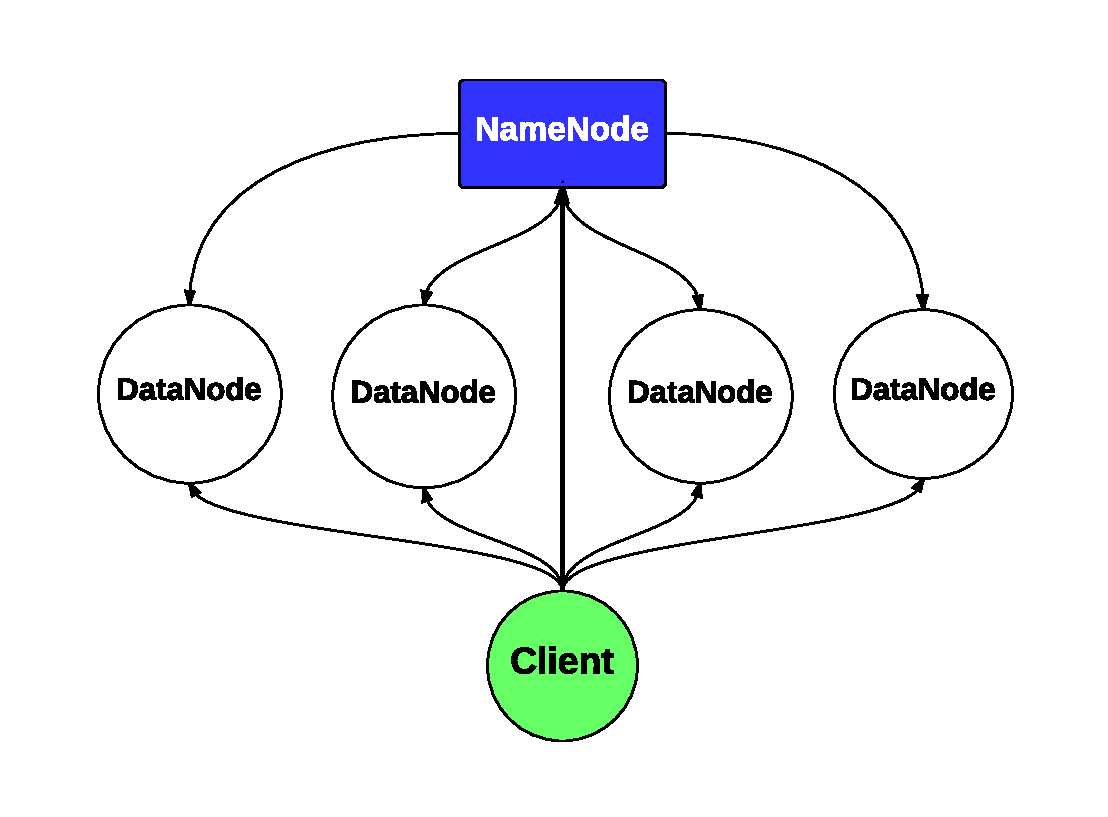
\includegraphics[scale=0.4]{assets/hadoop_architecture.pdf}
	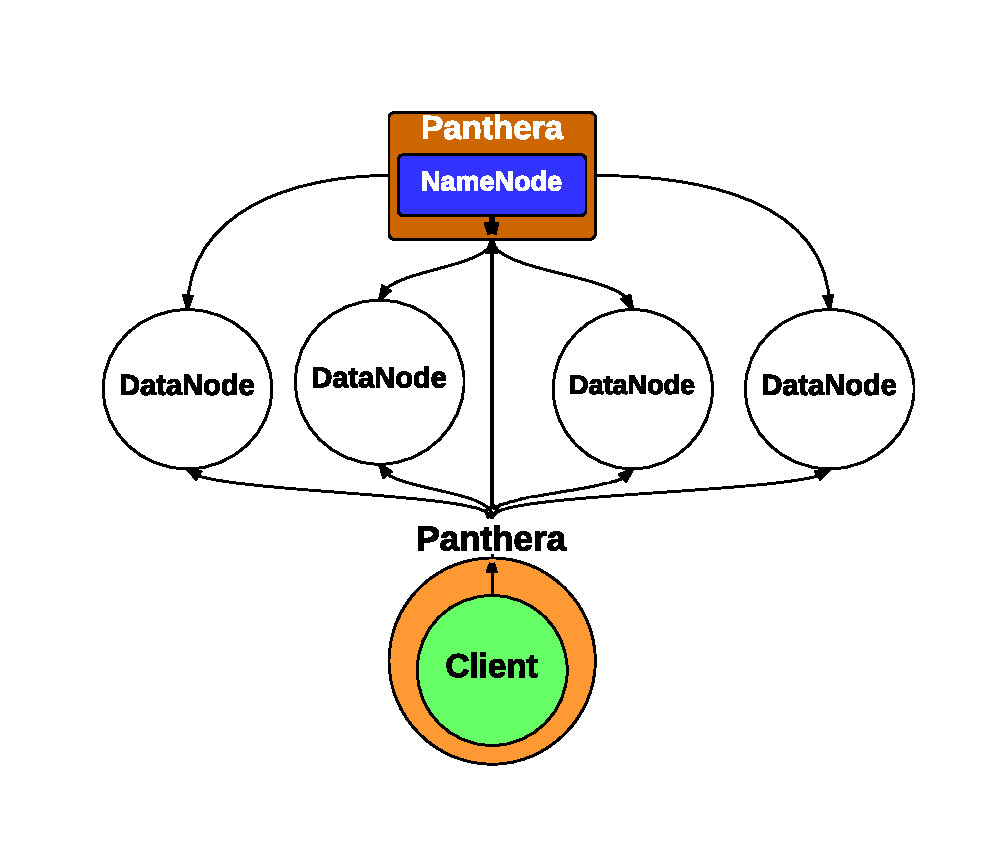
\includegraphics[scale=0.4]{assets/panthera_architecture.pdf}
\end{figure}

Figure 1 (see next page) outlines the architecture differences between a standard Hadoop File System architecture and an installation with Panthera. 

Within the standard conditions, the \textit{NameNode} serves as a metadata server, handling all requests from clients relating to metadata (e.g. directory listing, file sizes, block locations, etc.). \textit{DataNode(s)} hold data and serve it at request from the client. A more complete description of the Hadoop File System may be found in \cite{hadoop}.

Panthera operates by intercepting requests and responses at the NameNode and the client. Both nodes have a running instance of \textit{Panthera}. Every request issued from the client is first reviewed by Panthera, and if possible, answered immediately from the cache. The \textit{Panthera} instance on the NameNode constantly monitors the filesystem for changes that need to be reflected in the cache (e.g. if a file is deleted, the cache on the client should have a copy of it).

Panthera, since it caches both data and metadata, can be considered two separate subsystems, which are now discussed.

\section{Metadata caching}

\begin{figure}[!h]
	\caption{Panthera Metadata System}
	\centering
		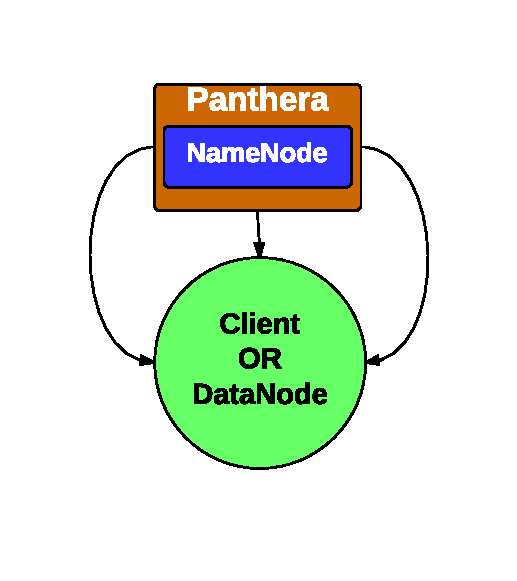
\includegraphics[scale=0.4]{assets/panthera_meta_architecture.pdf}
\end{figure}

The Panthera metadata system runs on the NameNode and communicates with the Panthera instance on the client. The challenge on the metadata portion consist of reducing computational latency to memory latency. For example, for some intensive methods (e.g. a recursive directory listing), it may be worthwhile to cache a response in order to prevent computing the same list again.

However, the problem lies in identifying such methods. Obviously, there are some methods for which caching is not worthwhile since their execution time is lower or comparable to memory latency. Within Panthera, six different Hadoop query methods were identified as medium to high latency. Panthera identifies packets that contain these methods and subsequently caches them.

Currently, a standard LRU cache \cite{cache} is used for each method. Testing of different caching methods and predictive prefetching algorithms is under way.

\section{Data caching}

\begin{figure}[!h]
	\caption{Panthera Data System}
	\centering
		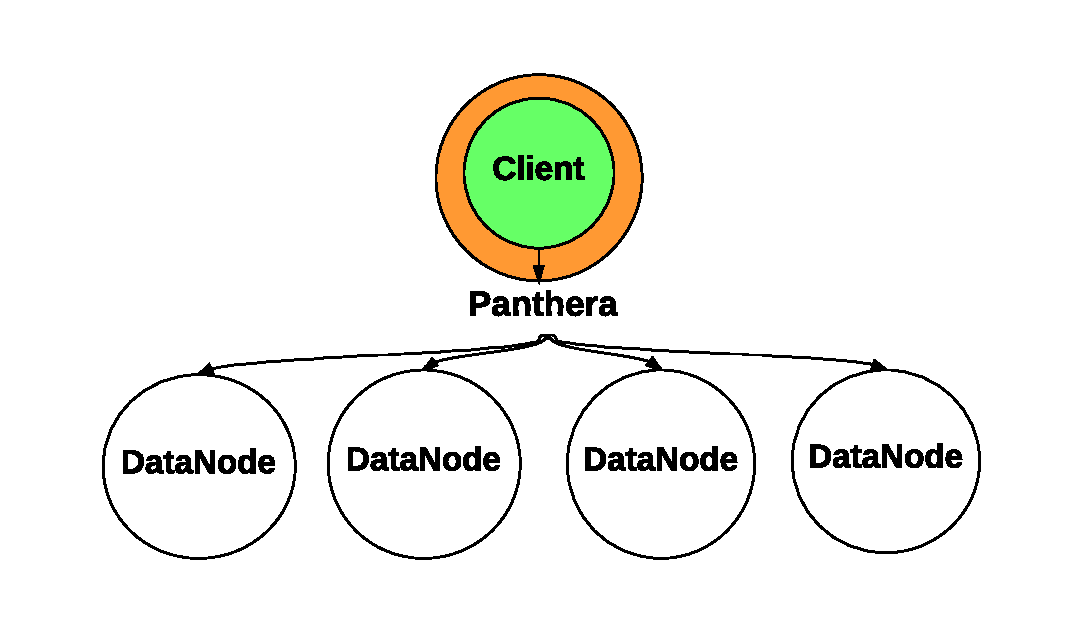
\includegraphics[scale=0.4]{assets/panthera_data_architecture.pdf}
\end{figure}

Panthera's data caching system runs on the client. The architecture is similar to that of the metadata caching system. Every request that the client makes to the DataNodes is first processed by Panthera and responded to from the cache if possible. 

The challenges with data caching differ significantly from those in metadata caching. Here, the goal is to convert network and hard drive read latency into memory latency. As \cite{ramcloud, hadoop} note, memory latency can be extremely low in modern systems, especially in comparison to network and hard drive latencies. Thus, in some respects, the goal is "easier" to attain in the data cache. However, for smaller files, it may be difficult to obtain latency improvement. 


\section{Testing Methodology}

In testing Panthera, very simple strategies were adopted. In order to test the metadata cache, a directory listing query was repeatedly run on a directory with 100 files in it, and the latency times for responding are measured, with Panthera and without. The reasoning for picking such a test lies in the fact that a directory listing in Hadoop involves all six of the cached methods as well as a few non-cached methods. Thus, the test provides a good estimate of the efficacy of the cache.

Latency times for the data cache were obtained by repeatedly querying for a one megabyte large file. The test encapsulates the most common use case for Panthera and the Hadoop File System.

Tests for the metadata cache were conducted on both single node and multinode setups, whereas the data cache testing was run on multinode setups.

\section{Results: Data caching}
\begin{figure}[!h]
	\caption{Panthera data cache latencies}
	\centering
		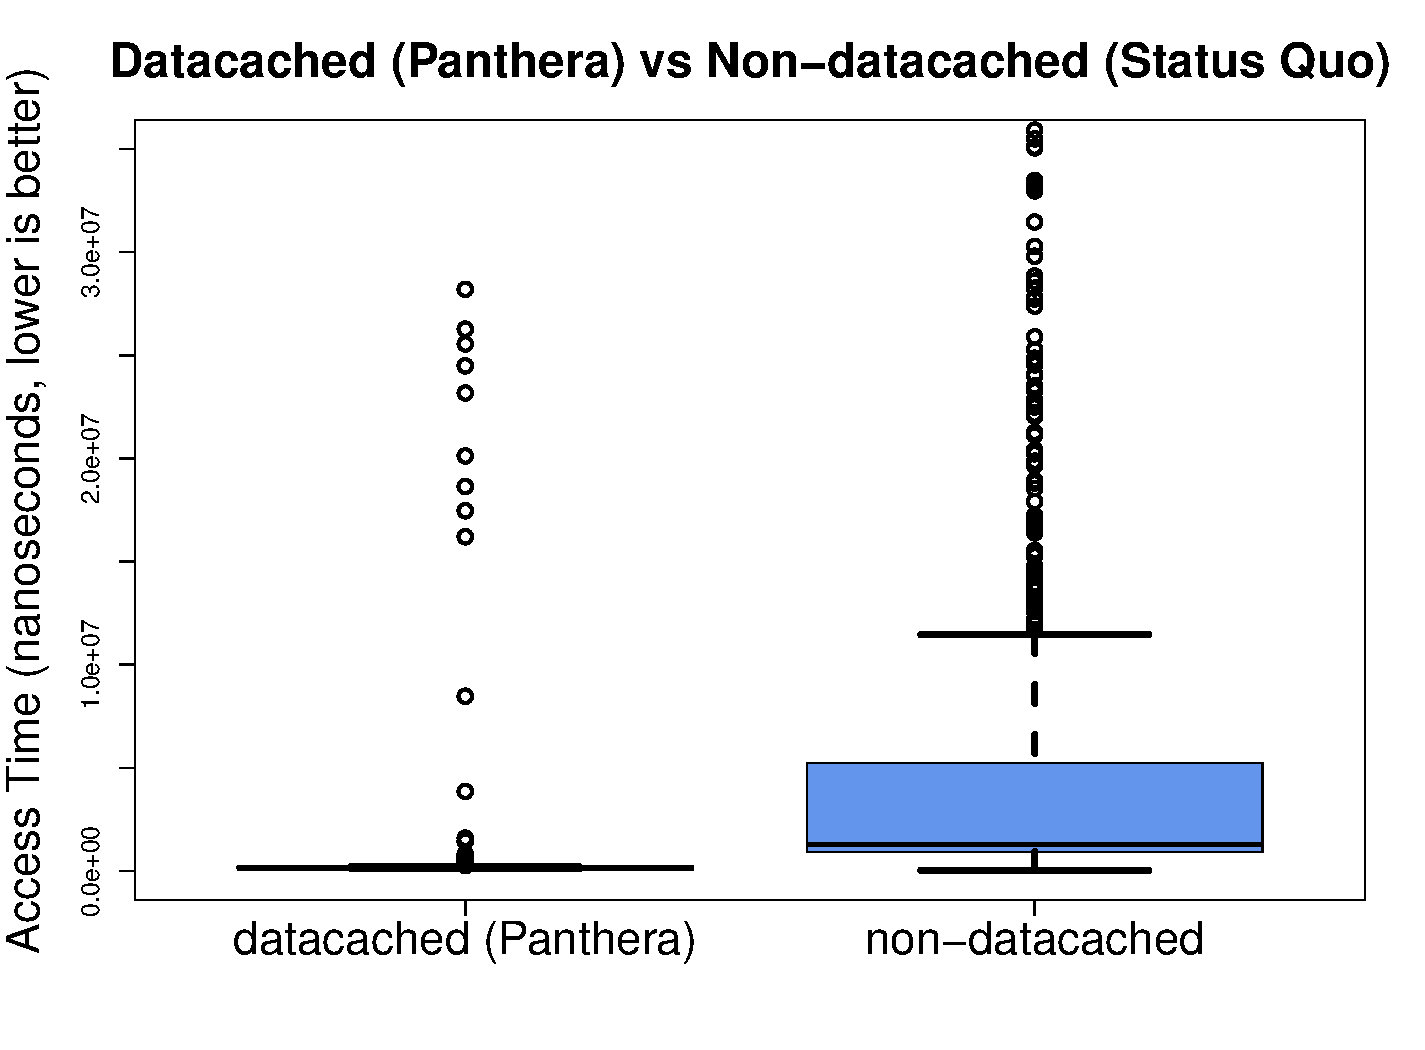
\includegraphics[scale=0.4]{assets/box-plot-data.pdf}
\end{figure}

\textbf{The Panthera data cache showed a 95.7\% decrease in the latency in comparison to a standard deviation non-datacached installation. In addition, the standard of deviation was lower by a factor of 27}. For any deployed project, maximum levels of latency must be considered when designing a system. Thus, the \textit{status quo} of the non-cached version severely limits possibilities within Hadoop. With \textit{Panthera}, not only is latency radically reduced, but also the variation in the latency is minimized.

\section{Results: Metadata caching}
\begin{figure}[!h]
	\caption{Panthera metadata cache latencies}
	\centering
		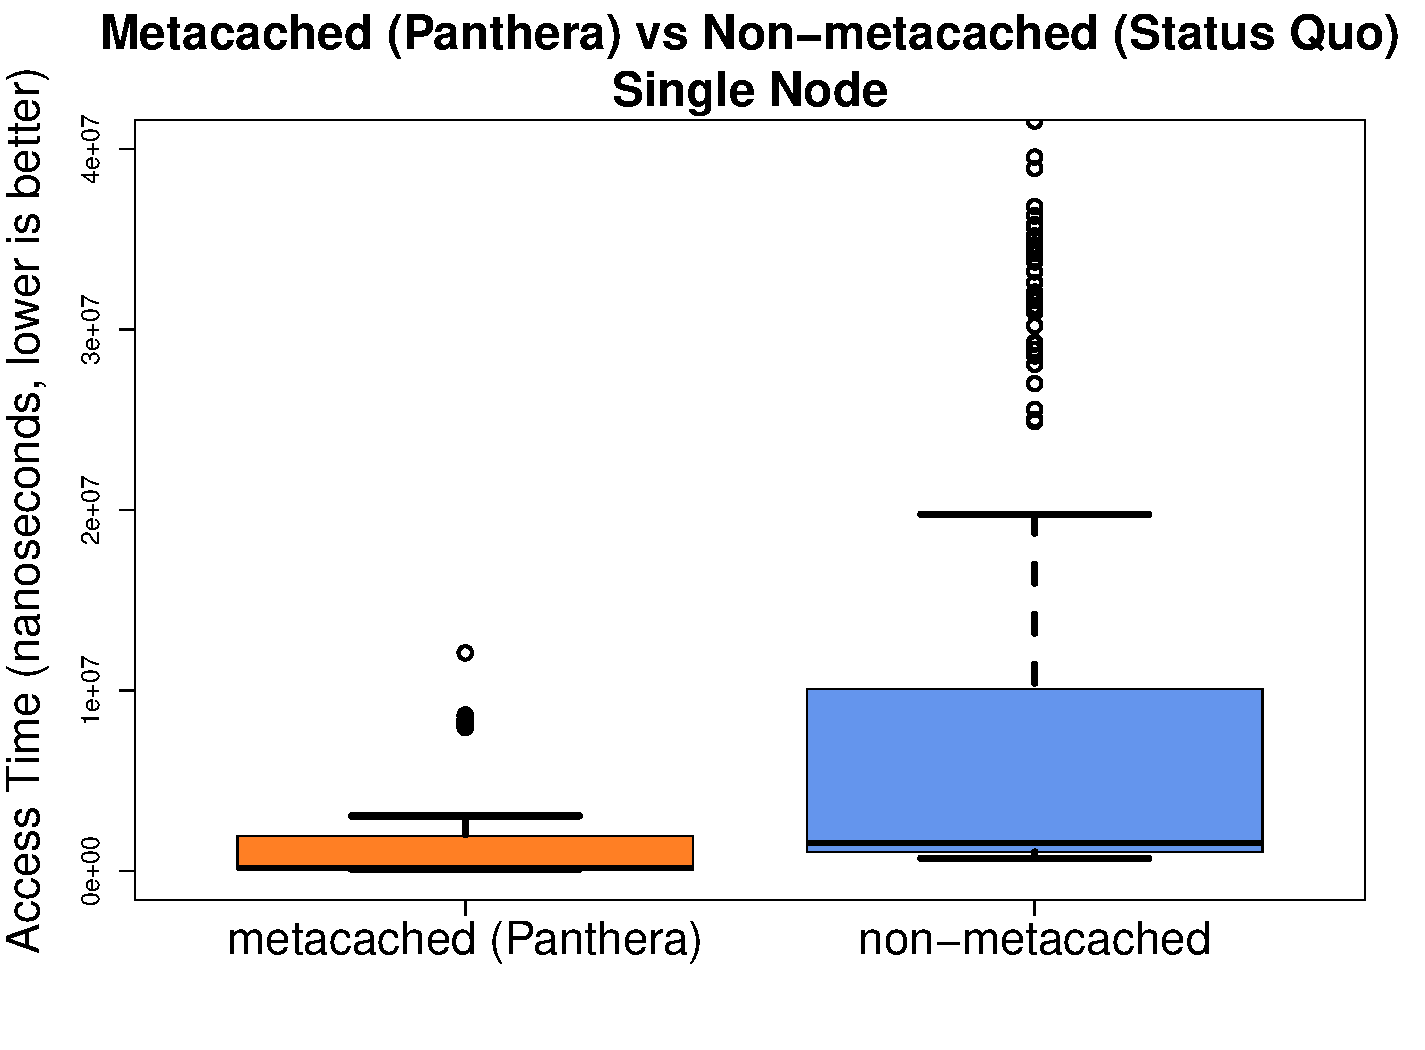
\includegraphics[scale=0.3]{assets/box-plot-metadata.pdf}
		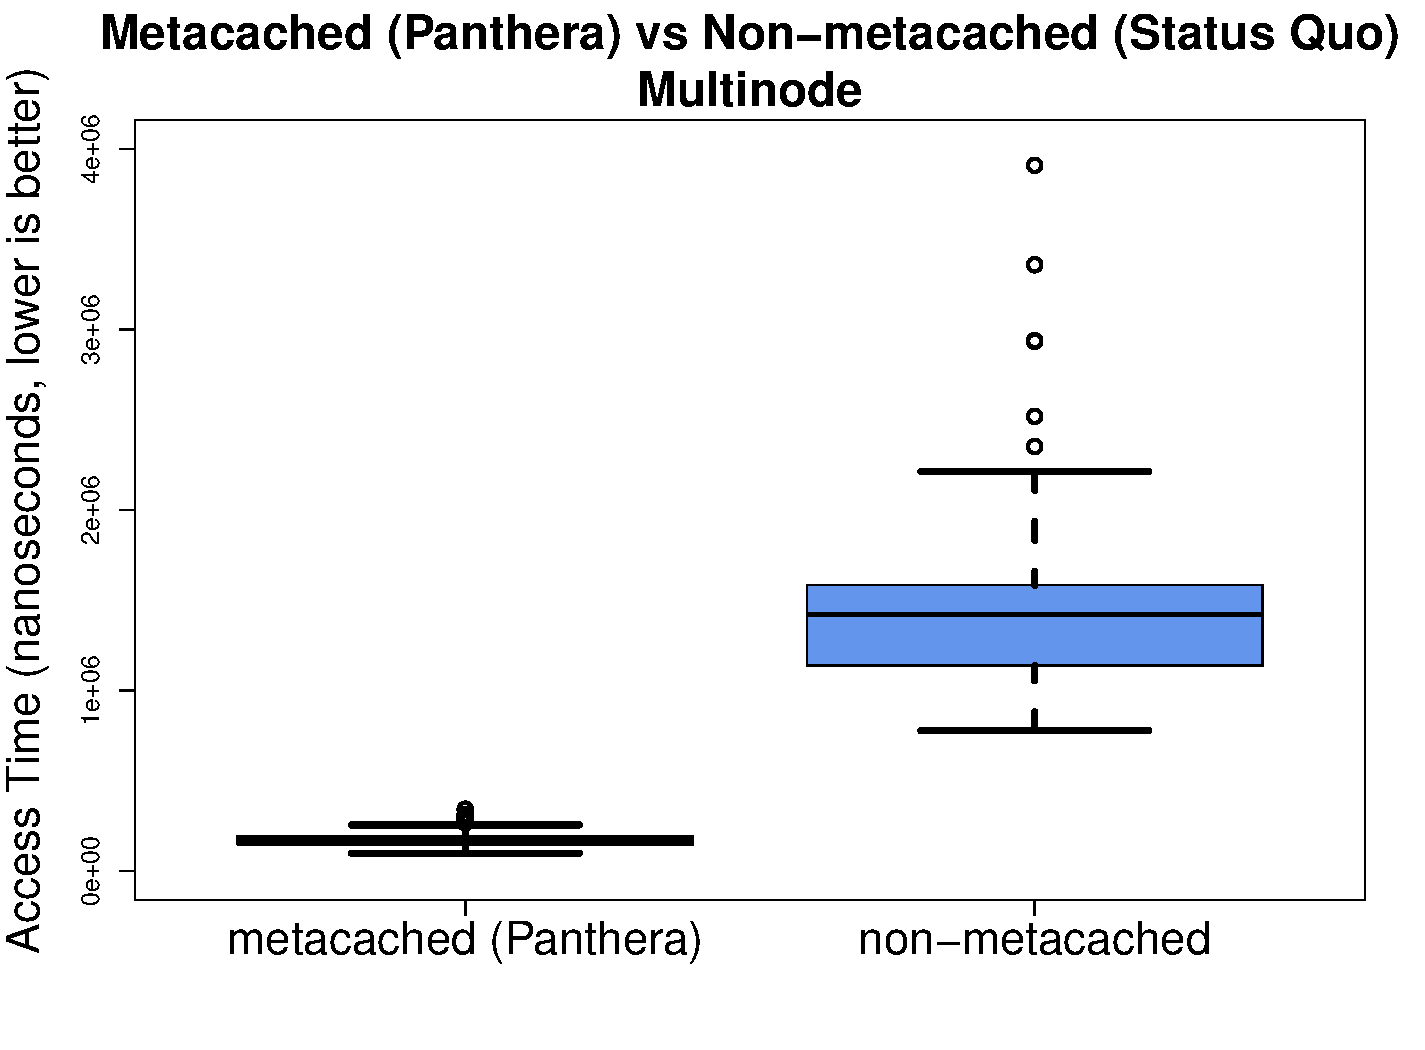
\includegraphics[scale=0.3]{assets/box-plot-metadata-multinode.pdf}
\end{figure}

Metadata caching has similarly incredible results. \textbf{\textit{Panthera} showed a 9 fold or 90.8\% improvement in the total latency as measured on the client side in a multinode setup}. Additionally, the standard deviation is 24 fold lower with\textit{Panthera}. Thus, this project has been able to minimize the latency averages as well as spreads to an extremely significant degree.

\section{Conclusion}

\textit{Panthera} fulfills the constraints mentioned at the outset. It is a layer on Hadoop rather than a main repository code modification. Considering the latency measurements, it is clear that it has also met the requirements in terms of benefit. \textit{Panthera} was able to reduce data access latency by 95.7\% and reduce basic metadata access latency by 90.8\%. Also, \textit{Panthera} was able to minimize the spread of latency times in both data and metadata requests. Thus, \textit{Panthera} opens up great possibilities within Hadoop due to the fact that algorithms that were previously impractical (e.g. distributed tree traversal algorithms) may now be implemented.

\section{Future work}
\textit{Panthera} can be extremely useful in a wide variety of applications, specifically in those which require large datasets in separate files (e.g. unstructured data). In particular, I will be concentrating on bioinformatics and integrating Panthera's caching with algorithms used in the area.

I am also working on a cache-based scheduler for Hadoop. Essentially, it will intelligently use information about what files are available in various clients and arrange Hadoop tasks such that the use of the cache is maximized.

Finally, all code associated with this paper and \textit{Panthera} will be open sourced in order to further development of Hadoop and distributed computing.

\nocite{*}

\bibliographystyle{plain}
\bibliography{references}

\end{document}